\documentclass[11pt,letterpaper]{article}

\newenvironment{proof}{\noindent{\bf Proof:}}{\qed\bigskip}

\newtheorem{theorem}{Theorem}
\newtheorem{corollary}{Corollary}
\newtheorem{lemma}{Lemma} 
\newtheorem{claim}{Claim}
\newtheorem{fact}{Fact}
\newtheorem{definition}{Definition}
\newtheorem{assumption}{Assumption}
\newtheorem{observation}{Observation}
\newtheorem{example}{Example}
\newcommand{\qed}{\rule{7pt}{7pt}}

\newcommand{\solution}[4]{
\thispagestyle{plain} 
\newpage
\setcounter{page}{1}
\noindent
\begin{center}
\framebox{ \vbox{
\vspace{4mm}
\vspace{0.2in} 
{\centering \large\mbox{#3}}\\
\vspace{0.1in}
{#1 \hfill {Date: #2}}
}}
\end{center}
\markright{#1}
}

\newenvironment{algorithm}
{\begin{center}
\begin{tabular}{|l|}
\hline
\begin{minipage}{1in}
\begin{tabbing}
\quad\=\qquad\=\qquad\=\qquad\=\qquad\=\qquad\=\qquad\=\kill}
{\end{tabbing}
\end{minipage} \\
\hline
\end{tabular}
\end{center}}

\def\Comment#1{\textsf{\textsl{$\langle\!\langle$#1\/$\rangle\!\rangle$}}}



\usepackage{graphicx, amssymb, amsmath, listings, float, mathtools}
\usepackage{color, url}
\lstset{language = Python}
\lstset{breaklines}
\lstset{extendedchars=false}

\oddsidemargin 0in
\evensidemargin 0in
\textwidth 6.5in
\topmargin -0.6in
\textheight 9.0in

\begin{document}

\solution{\large Jifu Zhao}{\large 03/25/2018}{\bf \Large STAT 578  \hspace{0.5cm} 
		Spring 2018 \hspace{0.5cm} Homework 2}

\section{Introduction}
Object recognition is a fundamental problem in computer vision. Even in a few years ago, it is still very hard for computers to automatically recognition cat versus dog. But now, with the development of deep learning algorithms, especially Convolutional Neural Networks (CNN), this task is much easier. In this project, using CIFAR10 dataset, I built two simple CNN models and try to recognize 10 different objects among a large amount of images.

CIFAR10 dataset is a collection of images that are commonly used to test computer vision algorithms for object recognition. It consists of 60,000 images in 10 different classes: airplane, automobile, bird, cat, deer, dog, frog, horse, ship, and truck. Each image is 32 $\times$ 32 $\times$ 3 RGB color image. A subset of 36 images from CIFAR10 dataset are shown in Fig.~\ref{fig:utility}.

% ---------------------------------------------------------------
\begin{figure}[htbp]
\centering
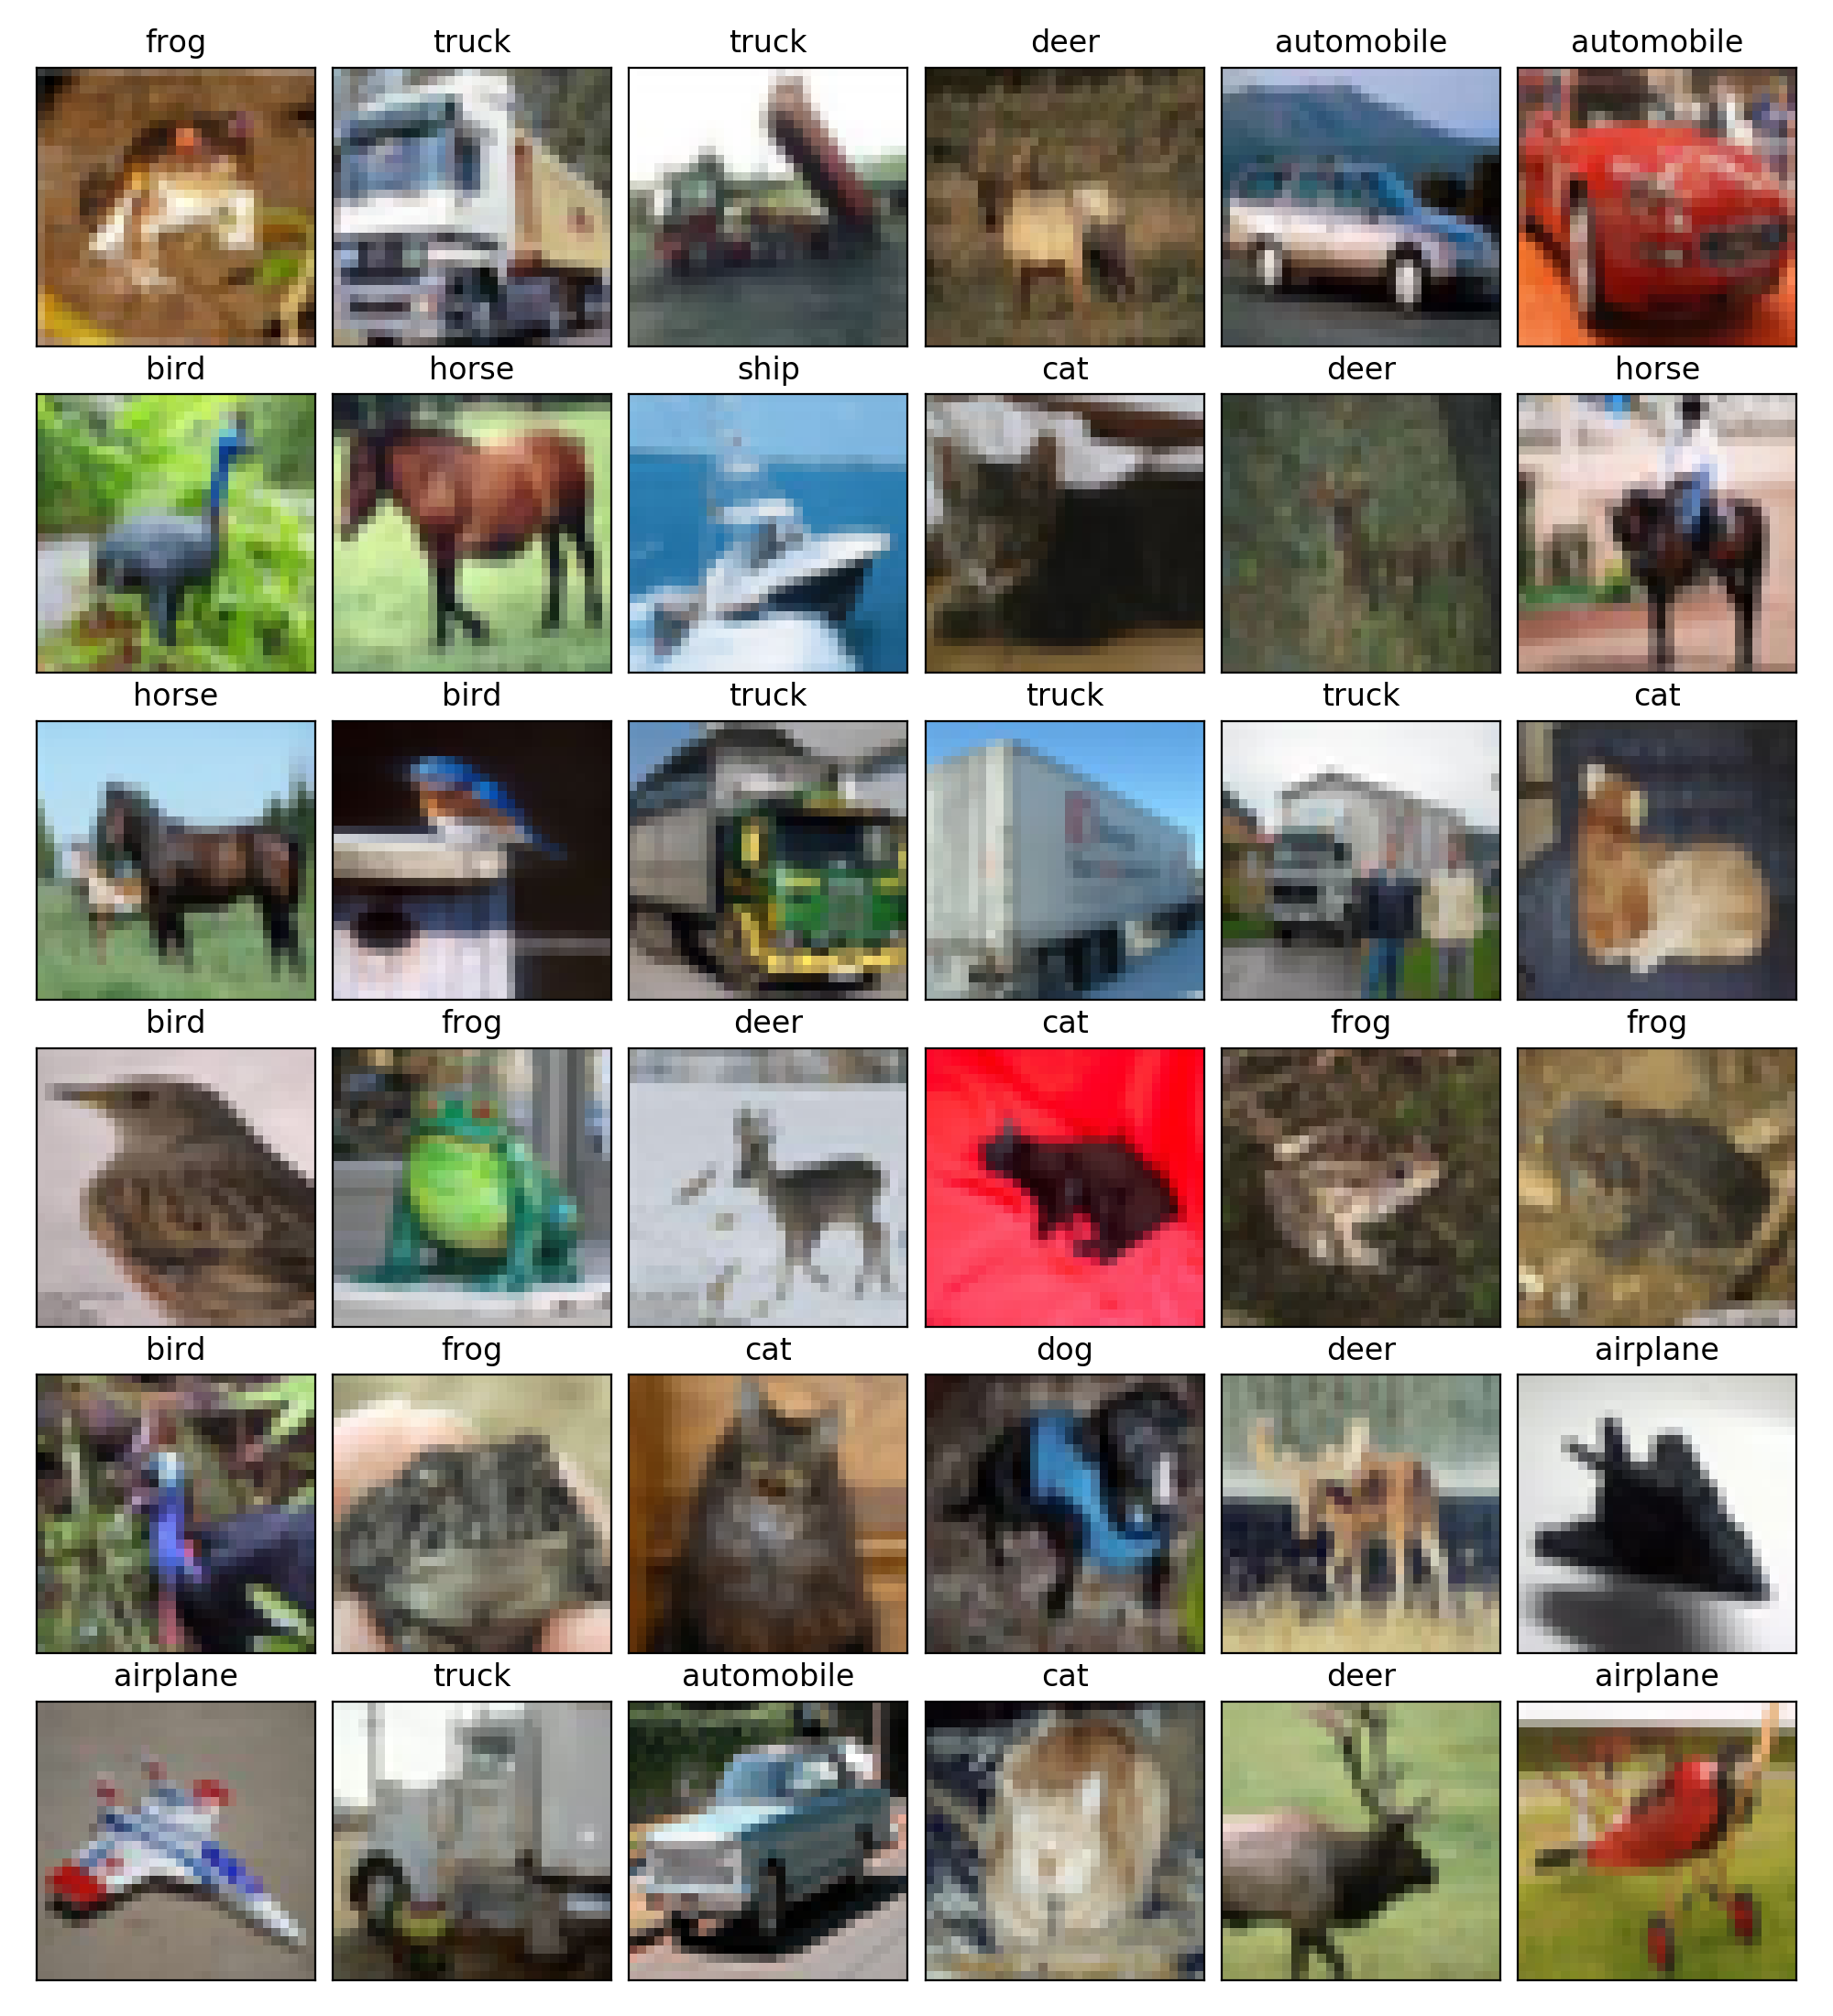
\includegraphics[width=0.70\textwidth]{./figures/snapshot.png}
\caption{Subset of CIFAR10 dataset.}
\label{fig:utility} 
\end{figure}


% ---------------------------------------------------------------
\section{CNN Models}
Recent years, there are a lot of different CNN models proposed for object recognition. Their performance has been tested on the famous ImageNet dataset. Fig.~\ref{fig:comparison} contains the comparison of different CNN models on ImageNet dataset. In this project, I implemented two widely used models: VGG and ResNet for object recognition on CIFAR10 dataset using Keras with TensorFlow.

% ---------------------------------------------------------------
\begin{figure}[htbp]
\centering
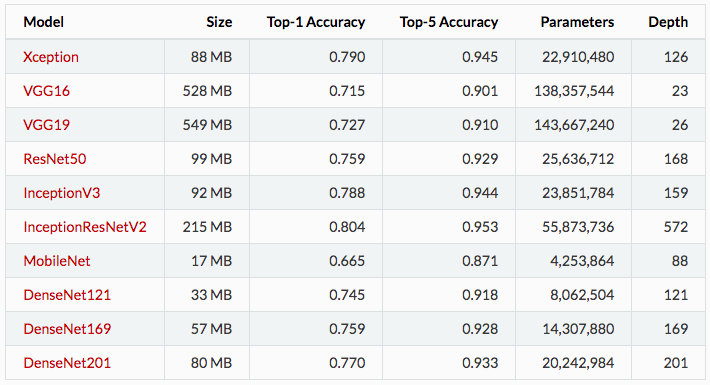
\includegraphics[width=0.9\textwidth]{./figures/comparison.png}
\caption{Comparison of different CNN models (Results come from keras.io).}
\label{fig:comparison} 
\end{figure}

\subsection{VGG}
VGG represents a series CNN models for computer vision tasks. It use a series of 3 $\times$ 3 convolution filters with different depths. VGG16 and VGG19 are the widely known models. An illustration of a sample VGG structure is shwon in Fig.~\ref{fig:vgg_sample}. In this project, instead of using deep VGG models like VGG16 or VGG19, I implemented a relatively shallow VGG model. The whole model structure is shown in Fig.~\ref{fig:vgg}.

% ---------------------------------------------------------------
\begin{figure}[htbp]
\centering
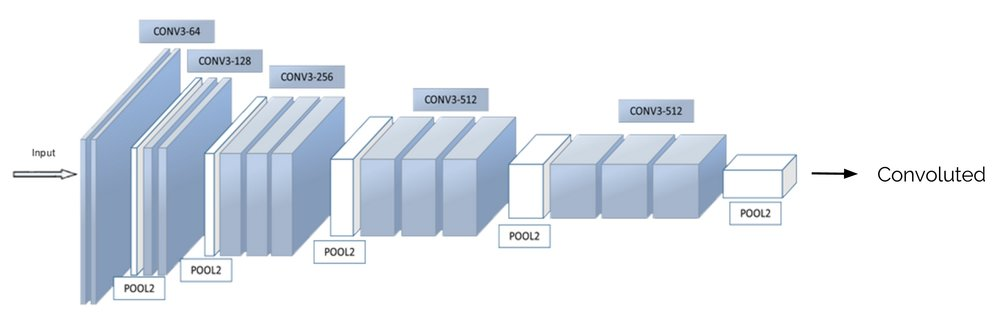
\includegraphics[width=0.9\textwidth]{./figures/vgg_image.jpeg}
\caption{Sample structure of VGG (image downloaded from Internet).}
\label{fig:vgg_sample} 
\end{figure}


% ---------------------------------------------------------------
\begin{figure}[htbp]
\centering
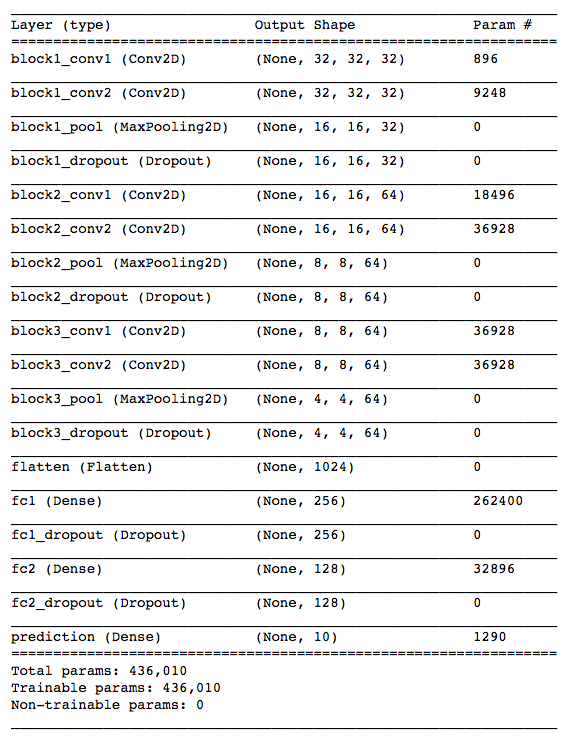
\includegraphics[width=1.0\textwidth]{./figures/vgg.png}
\caption{Structure of VGG.}
\label{fig:vgg} 
\end{figure}


\subsection{ResNet}
ResNet refers to the residual neural network structure. A sample ResNet model is shown in Fig.~\ref{fig:resnet_sample}. Through residual learning, ResNet can be built very large. For example, the original version on ImageNet has 156 layers. In this work, followed some online instruction, I build a relatively shallow ResNet model.

% ---------------------------------------------------------------
\begin{figure}[htbp]
\centering
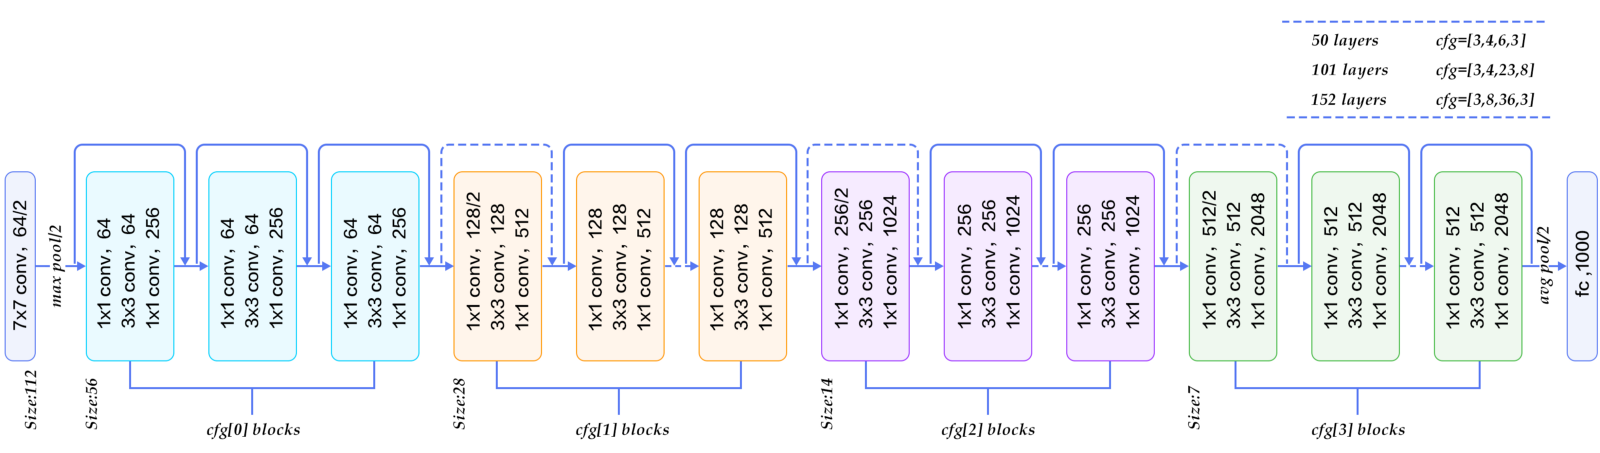
\includegraphics[width=1.0\textwidth]{./figures/resnet_image.png}
\caption{Sample structure of ResNet (image downloaded from Internet).}
\label{fig:resnet_sample} 
\end{figure}


\section{Results}

\subsection{VGG}
The training/validation loss and accuracy versus training epochs are shown in Fig.~\ref{fig:vgg_loss}. After 200 epochs, the test accuracy is around 0.85290, which is still underfit.

% ---------------------------------------------------------------
\begin{figure}[htbp]
\centering
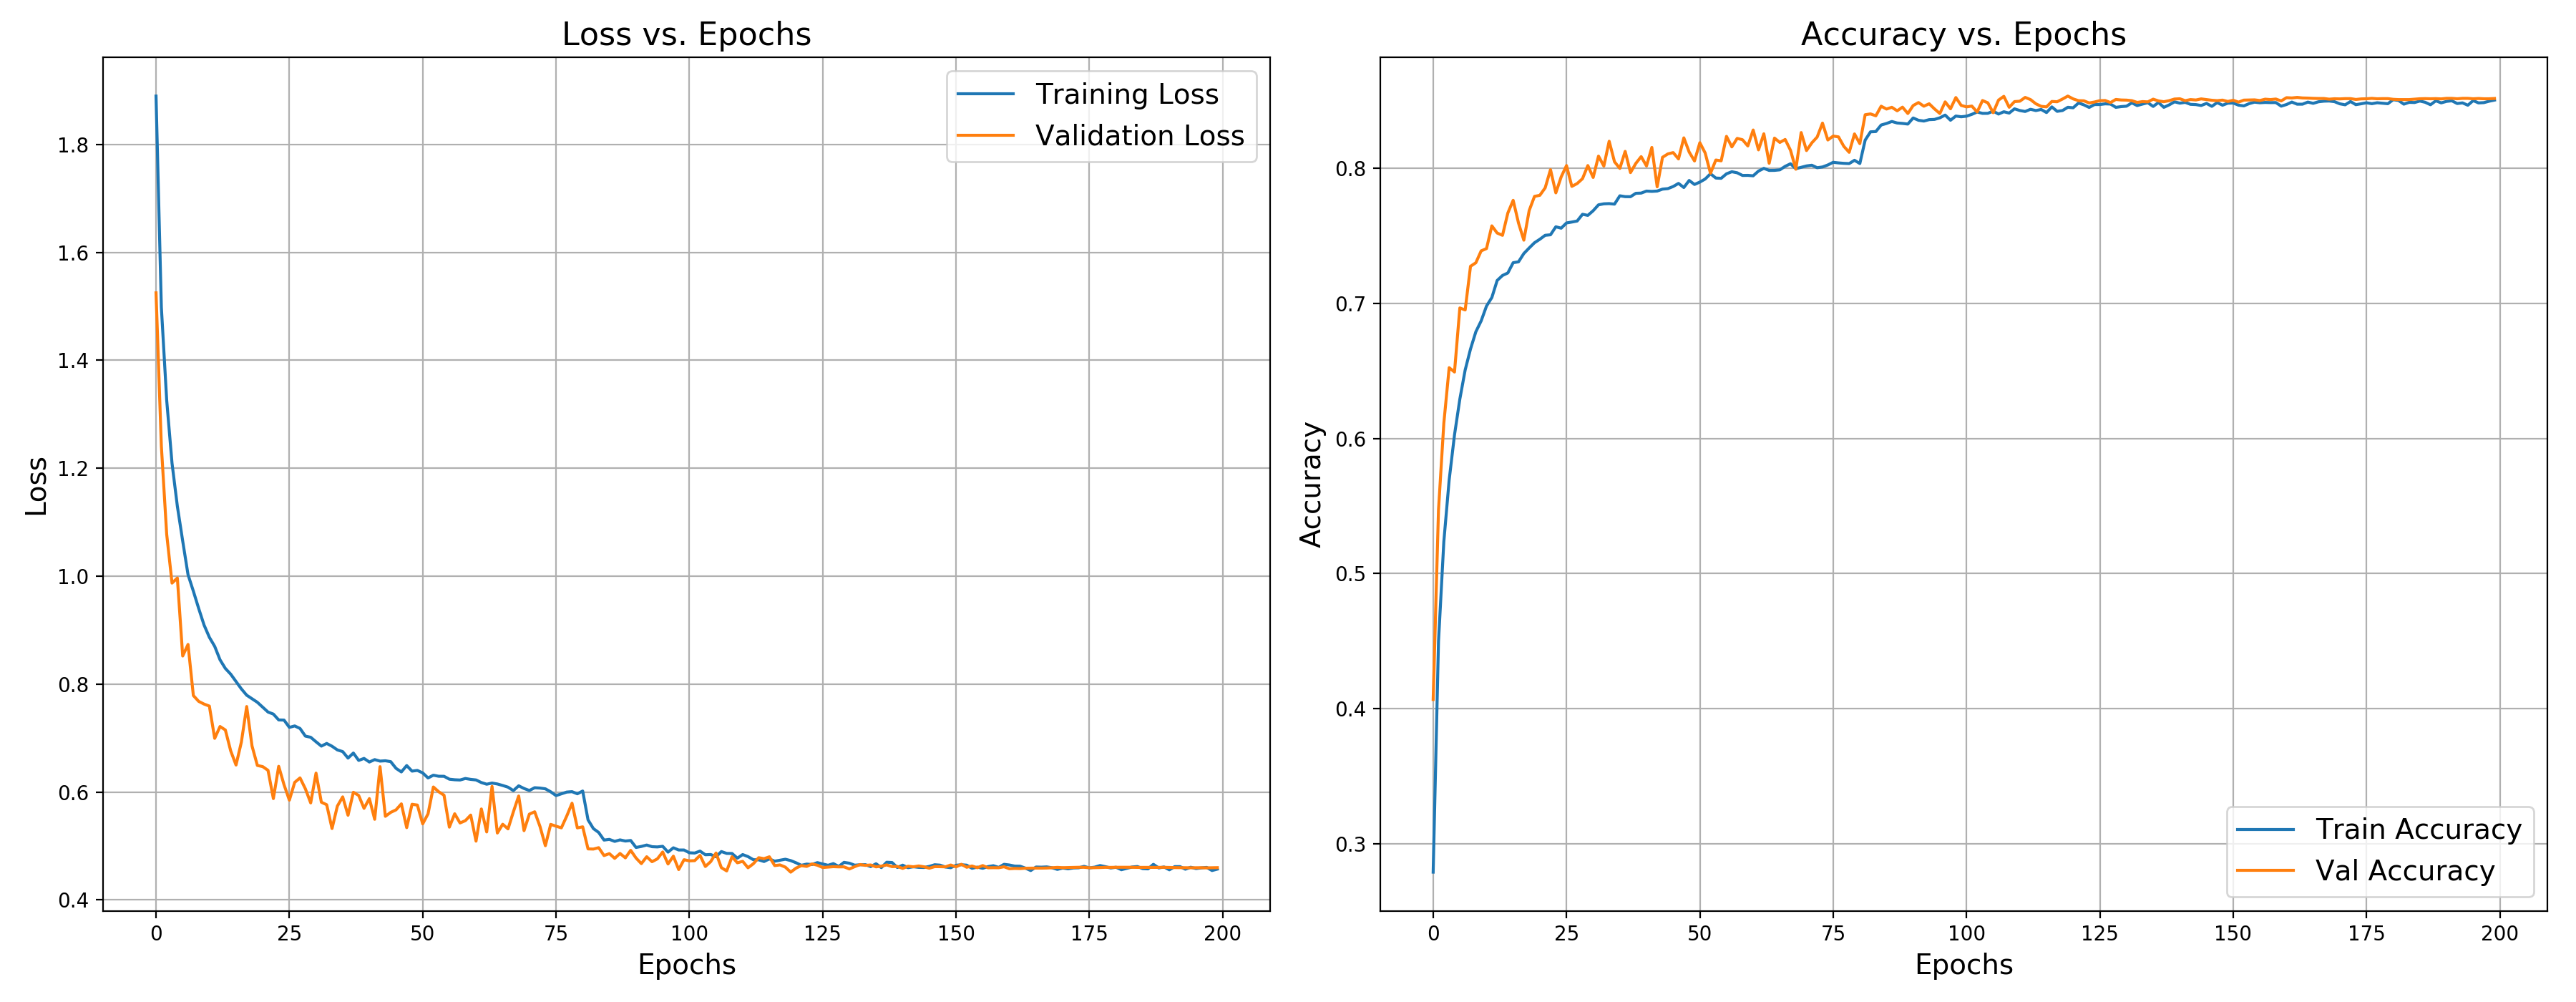
\includegraphics[width=1.0\textwidth]{./figures/vgg_loss.png}
\caption{Loss/Accuracy versus training epochs fro VGG.}
\label{fig:vgg_loss} 
\end{figure}



\subsection{ResNet}

The training/validation loss and accuracy versus training epochs are shown in Fig.~\ref{fig:resnet_loss}. After 200 epochs, the test accuracy is around 0.90840. Not a bad result, but the model seems to overfit a little bit.

% ---------------------------------------------------------------
\begin{figure}[htbp]
\centering
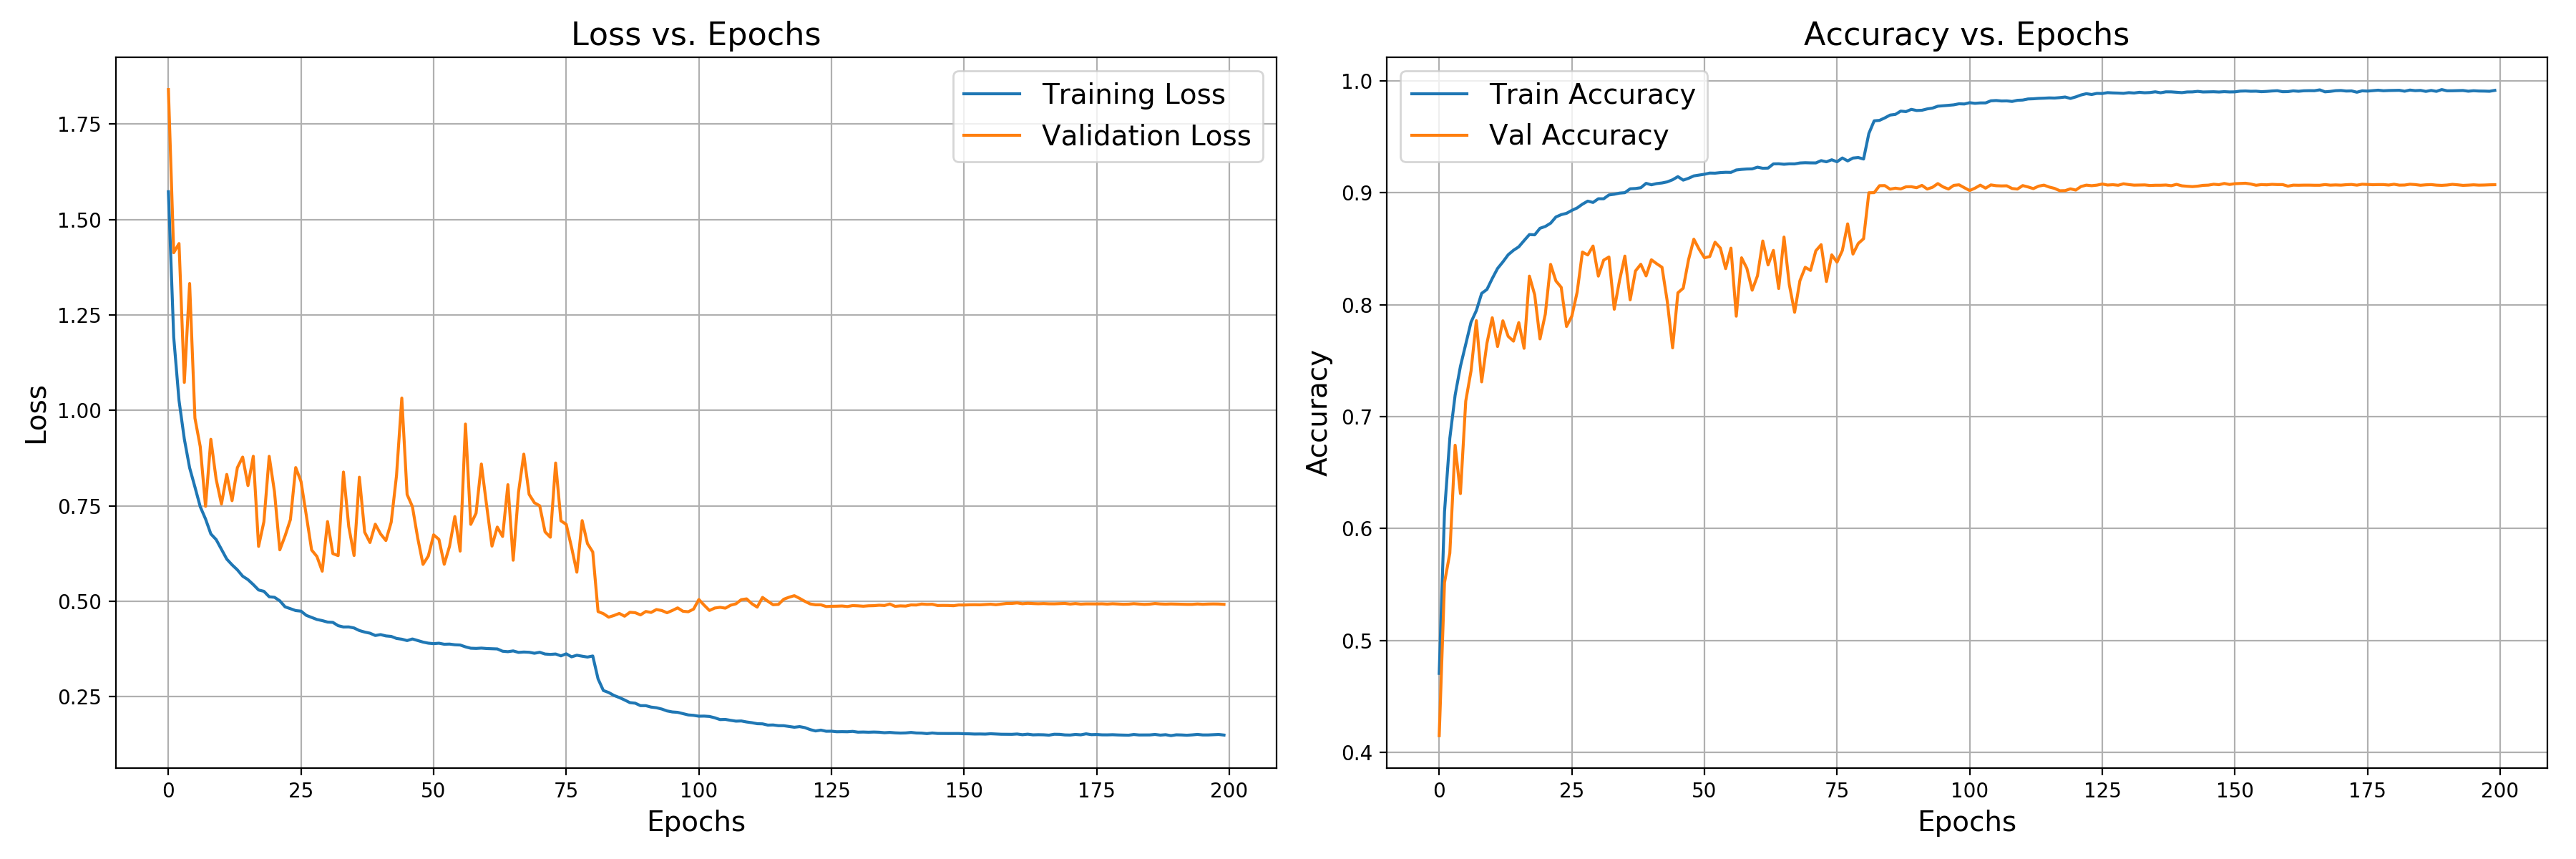
\includegraphics[width=1.0\textwidth]{./figures/resnet_loss.png}
\caption{Loss/Accuracy versus training epochs fro ResNet.}
\label{fig:resnet_loss} 
\end{figure}


Kaggle also holds a competition based on CIFAR10 dataset.  The result from ResNet are among the top 20 based on the historical data.


\clearpage

%\bibliographystyle{plain}
%\bibliographystyle{unsrt}
%\bibliography{reference.bib}

\end{document}

